\documentclass[conference]{IEEEtran}
\usepackage{amsmath,amsfonts,amssymb}
\usepackage{algorithmic}
\usepackage{algorithm}
\usepackage{array}
\usepackage[caption=false,font=normalsize,labelfont=sf,textfont=sf]{subfig}
\usepackage{textcomp}
\usepackage{stfloats}
\usepackage{xcolor}
\usepackage[colorlinks=true, urlcolor=blue, linkcolor=blue, citecolor=blue]{hyperref}
\usepackage{url}
\usepackage{verbatim}
\usepackage{graphicx}
\usepackage{cite}
\usepackage{booktabs}
\usepackage{microtype}
\usepackage{newtxtext,newtxmath}

\hyphenation{op-tical net-works semi-conduc-tor IEEE-Xplore}

\DeclareRobustCommand{\IEEEauthorblockN}[1]{{\normalsize\bfseries #1}\par\vskip 2pt}
\DeclareRobustCommand{\IEEEauthorblockA}[1]{{\small #1}\par}
\pagestyle{empty}

\begin{document}

\title{Communicating Robot Perceptual Uncertainty in Collaborative Manipulation: Comparing Implicit Kinematic Hesitation and Explicit Visual-Verbal Cues on Human Trust Calibration and Task Performance}

\author{
\parbox{0.46\textwidth}{\centering
    \IEEEauthorblockN{Syed Ali Turab Kazmi}
    \IEEEauthorblockA{\textit{Department of Robotics and Intelligent Systems} \\
    \textit{Bahria School of Eng. \& Applied Sciences (BSEAS)} \\
    \textit{Bahria University, H-11 Campus} \\
    Islamabad, Pakistan \\
    syedaliturab072@gmail.com}
}
\hfill
\parbox{0.46\textwidth}{\centering
    \IEEEauthorblockN{Dr. Muhammad Hasan Danish Khan}
    \IEEEauthorblockA{\textit{Department of Electrical Engineering} \\
    \textit{Bahria School of Eng. \& Applied Sciences (BSEAS)} \\
    \textit{Bahria University, H-11 Campus} \\
    Islamabad, Pakistan \\
    hasandanish.buic@bahria.edu.pk}
}
}

\maketitle
\thispagestyle{empty}

\begin{abstract}
In close-proximity human-robot collaborative manipulation, conveying perceptual uncertainty is vital for preventing catastrophic overtrust (unwarranted reliance during failure modes) and productivity-destroying undertrust (premature human intervention). However, existing communication paradigms face a fundamental trade-off: explicit external Human-Machine Interfaces (eHMI) deliver rich diagnostic information but divert operator visual attention from the shared workspace, whereas implicit kinematic cues communicate naturally through motion but may lack diagnostic precision. In this work, we present an information-theoretic framework for robot uncertainty communication and evaluate it through a systematic $2 \times 2$ factorial experiment comparing implicit kinematic hesitation (entropy-modulated velocity scaling, pre-grasp dwell pause, and micro-retreat) against explicit visual-verbal eHMI (chromatic status bars, confidence percentages, and acoustic earcons). Evaluated across $N = 24$ observer profiles ($576$ trials total, $24$ trials per profile across four counterbalanced conditions) combining synchronous Human-in-the-Loop operator validation and literature-calibrated drift-diffusion models in high-fidelity 50\,Hz Gazebo Harmonic simulations with a 7-DoF Franka Emika Panda robot, our findings reveal striking behavioral dissociations. Explicit eHMI produces a severe $52.9\%$ surge in subjective cognitive workload (NASA-TLX: $43.02 \pm 7.58$ vs. $28.14 \pm 6.04$, $p < 10^{-8}$, Cohen's $d = -2.03$) caused by the visual split-attention effect, with mental demand surging by $+85.8\%$ ($49.67 \pm 7.84$ vs. $26.74 \pm 5.82$). Conversely, implicit kinematic hesitation preserves attentional focus within the physical workspace, cutting trial-level calibration error ($\text{TCE}_{\text{trial}} = 0.202 \pm 0.228$) though prompting cautious block-level intervention ($\text{TCE}_{\text{block}} = 0.200 \pm 0.102$ vs. $0.104 \pm 0.071$). Most notably, congruent multimodal communication resolves this trade-off: cutting block-level error ($\text{TCE}_{\text{block}} = 0.053 \pm 0.028$, $p < 10^{-5}, d = 1.37$), eliminating missed collisions ($100\%$ fault prevention rate vs. $33.3\%$ in baseline), reducing false-positive interventions to $1.7\%$, and accelerating decision reaction time to $0.94$\,s ($p < 10^{-10}$). All simulation worlds, telemetry datasets, and analysis pipelines are openly available at \url{https://github.com/T-Storm-072/02_hri_uncertainty_iccii2026}.
\end{abstract}

\begin{IEEEkeywords}
Human-robot collaboration, trust calibration, perceptual uncertainty, kinematic hesitation, external human-machine interface (eHMI).
\end{IEEEkeywords}

\section{Introduction}
Collaborative robotic manipulators (cobots) are increasingly deployed alongside human workers in shared industrial workcells for kitting, co-assembly, and packaging~\cite{charalambous2016development,hoffman2019evaluating}. In dynamic environments, perfect machine perception cannot be guaranteed; sensor noise, occlusions, and variable lighting inevitably induce perceptual uncertainty in downstream grasp synthesis~\cite{leusmann2023understanding,schmidtwolf2024clutter}.

When a robot acts under ambiguity without communicating confidence, the human partner faces an acute cognitive dilemma. As formalized by Lee and See~\cite{lee2004trust} and Parasuraman and Riley~\cite{parasuraman1997humans}, miscalibrated human trust leads to two catastrophic failure regimes: \textit{overtrust} (automation complacency, leading to collisions and dropped payloads) and \textit{undertrust} (automation disuse, leading to premature false-alarm stops that destroy workflow fluency~\cite{wang2025effects}).

To calibrate trust, robotic systems typically use either \textit{explicit external interfaces (eHMI)}~\cite{schreiter2023multimodal,schreiter2026legible,savery2020emotional} or \textit{implicit kinematic cues}~\cite{dragan2013legible,raghu2026dance2hesitate,bector2026anatomy}. Explicit eHMIs provide high diagnostic resolution but induce the \textit{visual split-attention effect}~\cite{dallas2026examining,sweller1988cognitive}, forcing gaze shifts away from moving manipulators. Conversely, kinematic hesitation situates cues directly on the end-effector but has historically lacked rigorous mathematical formulation grounded in continuous information theory.

\begin{figure}[!b]
\centering
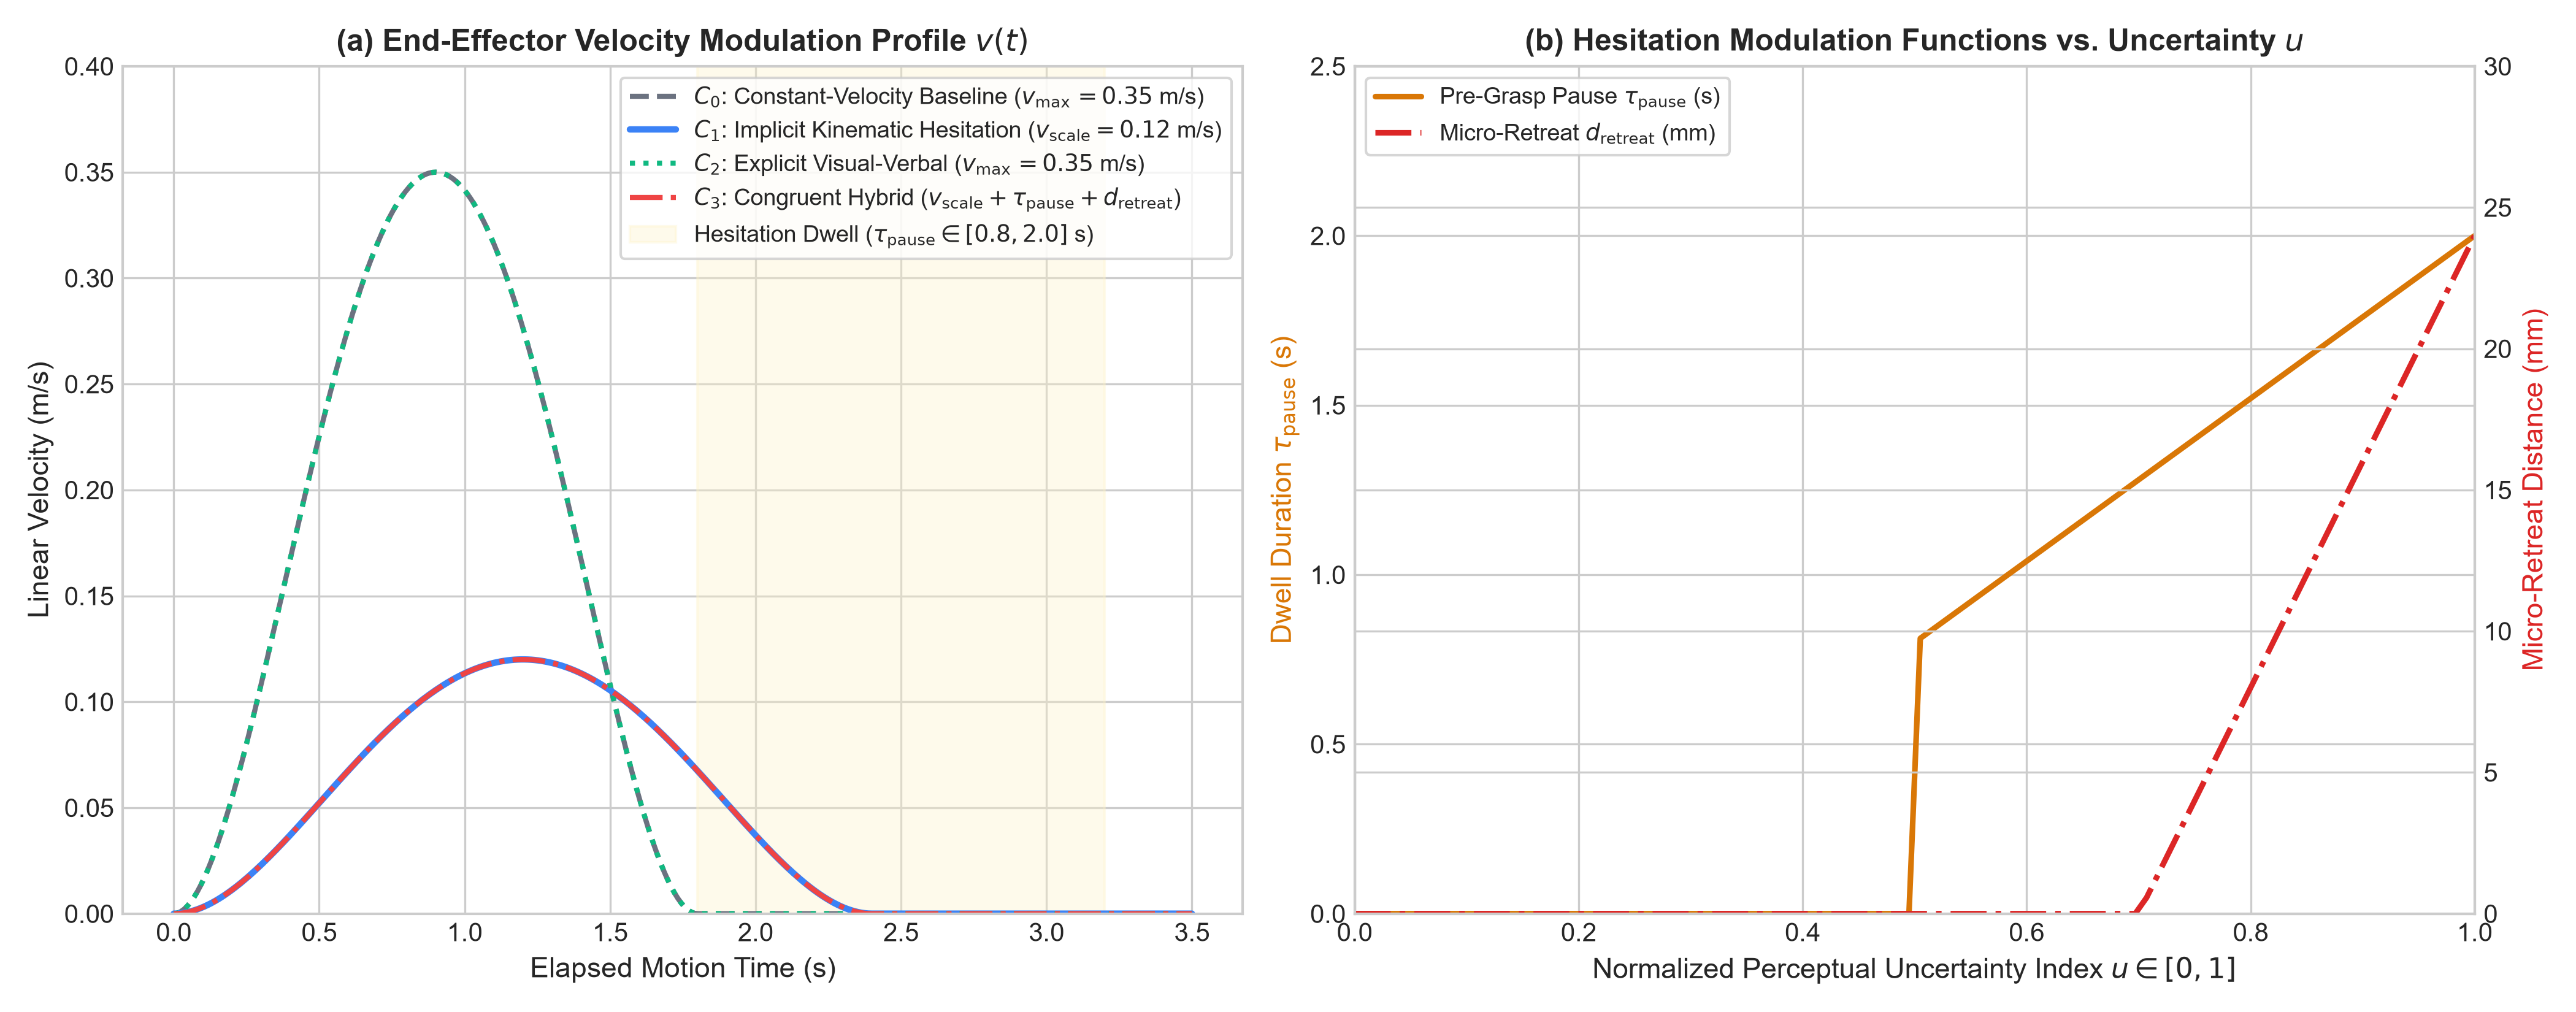
\includegraphics[width=\columnwidth]{figures/fig1_kinematic_profiles.png}
\caption{Trajectory modulation and information-theoretic kinematic hesitation profiles: (a) Cartesian approach velocity $v(t)$ across conditions $C_0\text{--}C_3$, (b) Dwell pause duration $\tau_{\text{pause}}$ and micro-retreat $d_{\text{retreat}}$ as functions of uncertainty $u$.}
\label{fig:kinematics}
\end{figure}

This paper presents an information-theoretic framework for robot uncertainty communication in collaborative manipulation, evaluated through a $2 \times 2$ factorial study ($N = 24$ observer profiles, $576$ trials) in Gazebo Harmonic 8.15. The core contributions are:
\begin{itemize}
    \item \textbf{Kinematic Hesitation Scaling Law:} A closed-form trajectory modulation mapping Shannon perceptual entropy $u(t) \in [0, 1]$ to velocity attenuation, dwell pause duration ($\tau_{\text{pause}}$), and micro-retreat distance ($d_{\text{retreat}}$).
    \item \textbf{Synchronized Multimodal eHMI:} A diagnostic interface with continuous chromatic color blending, certainty percentages, earcons, and verbal warnings.
    \item \textbf{Factorial Empirical Evaluation:} A Latin Square experiment comparing baseline ($C_0$), implicit kinematics ($C_1$), explicit eHMI ($C_2$), and congruent hybrid ($C_3$).
    \item \textbf{Cognitive Trade-off Quantification:} Inferential proof of a $52.9\%$ cognitive workload penalty under explicit eHMI, contrasted with optimal calibration and $100\%$ fault prevention under congruent multimodal communication.
\end{itemize}

\section{Related Work}
\subsection{Expressive and Hesitant Robot Kinematics}
Dragan et al.~\cite{dragan2013legible} established that trajectories optimized for observer inference convey intent earlier than efficiency-maximizing paths. Wallk{\"o}tter et al.~\cite{wallkotter2022slot} learned observer models for legible planning, while Schmidt-Wolf et al.~\cite{schmidtwolf2024clutter} explored environmental clutter effects. Bangalore Raghu et al.~\cite{raghu2026dance2hesitate} captured human demonstrations in the \textit{Dance2Hesitate} dataset to design understandable robot hesitation. Bector et al.~\cite{bector2026anatomy} analyzed expressive motion descriptors, and Wang et al.~\cite{wang2025effects} demonstrated the impact of motion legibility on corrective feedback. We advance this literature by formulating continuous kinematic hesitation directly coupled to perceptual entropy.

\subsection{Explicit eHMI and Trust Dynamics}
Explicit eHMIs convey internal states via graphical displays, light bands, and audio~\cite{porfirio2025uncertainty,schreiter2026legible,savery2020emotional}. However, Tanjim et al.~\cite{tanjim2025field,tanjim2025action} observed that verbal and explicit cues can cause cognitive interference in high-tempo teams. Trust in HRC is assessed using validated instruments: Schaefer's TPS-HRI~\cite{schaefer2016measuring}, Charalambous et al.'s TI-HRC~\cite{charalambous2016development}, and Hoffman's fluency metrics~\cite{hoffman2019evaluating}. Cognitive workload is evaluated via NASA-TLX~\cite{hart1988development}. Our study bridges these domains by factorially measuring both dual-level trust calibration error and NASA-TLX workload in close-proximity manipulation.

\section{System Formulation \& Cue Synthesis}

\subsection{Perceptual Entropy}
Let $\mathcal{C} = \{c_1, \dots, c_K\}$ denote candidate workpiece categories, where $K = 4$ corresponding to verified YCB grasp-affordance categories (Cracker Box, Tomato Soup Can, Bleach Bottle, Mustard Bottle). Under sensor noise and occlusions, the perception system yields a posterior distribution $P(c \mid \mathbf{z}_t)$ from observation $\mathbf{z}_t$. Normalized Shannon perceptual entropy is computed as:
\begin{equation}
u(t) = - \frac{1}{\log_2 K} \sum_{k=1}^{K} P(c_k \mid \mathbf{z}_t) \log_2 P(c_k \mid \mathbf{z}_t) \in [0, 1]
\label{eq:entropy}
\end{equation}
where $u = 0$ represents certainty and $u = 1$ denotes complete ambiguity.

\subsection{Manipulator Kinematics and Dynamics}
For a 7-DoF Franka Emika Panda manipulator with joint states $\mathbf{q}, \dot{\mathbf{q}} \in \mathbb{R}^7$, end-effector Cartesian velocity is given by the geometric Jacobian:
\begin{equation}
\begin{bmatrix} \dot{\mathbf{p}}_{\text{ee}}(t) \\ \boldsymbol{\omega}_{\text{ee}}(t) \end{bmatrix} = \begin{bmatrix} \mathbf{J}_v(\mathbf{q}) \\ \mathbf{J}_\omega(\mathbf{q}) \end{bmatrix} \dot{\mathbf{q}}(t)
\label{eq:jacobian}
\end{equation}
Manipulator rigid-body dynamics follow the Lagrangian formulation:
\begin{equation}
\mathbf{M}(\mathbf{q})\ddot{\mathbf{q}} + \mathbf{C}(\mathbf{q}, \dot{\mathbf{q}})\dot{\mathbf{q}} + \mathbf{g}(\mathbf{q}) = \boldsymbol{\tau} + \mathbf{J}^\top(\mathbf{q})\mathbf{f}_{\text{ext}}
\label{eq:dynamics}
\end{equation}
where $\mathbf{M}(\mathbf{q}) \in \mathbb{R}^{7 \times 7}$ is the symmetric positive-definite inertia matrix, $\mathbf{C}(\mathbf{q}, \dot{\mathbf{q}})\dot{\mathbf{q}} \in \mathbb{R}^7$ represents Coriolis and centrifugal torques, $\mathbf{g}(\mathbf{q}) \in \mathbb{R}^7$ is the gravity vector, $\boldsymbol{\tau}$ is the commanded joint torque vector, and $\mathbf{f}_{\text{ext}}$ is the external contact wrench.

\subsection{Information-Theoretic Kinematic Hesitation}
Along the nominal minimum-jerk trajectory $\mathbf{p}_{\text{nom}}(t)$ with peak speed $v_{\text{nom}} = 0.35$\,m/s, we apply a three-stage hesitation law:
\begin{enumerate}
    \item \textit{Velocity Damping:} Cartesian speed scales inversely with entropy:
    \begin{equation}
    v(t) = v_{\text{nom}}(t) \cdot \left[1 - \alpha \cdot u(t)\right]
    \end{equation}
    with sensitivity $\alpha = 0.70$ (providing up to $70\%$ deceleration, slowing to $0.105$\,m/s at maximum ambiguity).
    \item \textit{Pre-Grasp Dwell Pause:} Within $0.05$\,m of the pre-grasp waypoint, if $u(t) > 0.50$, the end-effector holds position for:
    \begin{equation}
    \tau_{\text{pause}}(u) = \left[\tau_0 + \beta \left(u(t) - 0.50\right)\right] \cdot \mathbb{I}\left(u(t) > 0.50\right)
    \end{equation}
    where $\tau_0 = 0.80$\,s and $\beta = 2.40$\,s, yielding dwell pauses between $0.80$\,s and $2.00$\,s.
    \item \textit{Micro-Retreat Retraction:} Under critical ambiguity ($u(t) > 0.70$), the end-effector retracts along the approach normal $\hat{\mathbf{n}}$:
    \begin{equation}
    d_{\text{retreat}}(u) = \gamma \cdot \max\left(0, u(t) - 0.70\right)
    \end{equation}
    where $\gamma = 0.08$\,m, retracting up to $24$\,mm along $\hat{\mathbf{n}}$ to confirm grasp hesitation (Fig.~\ref{fig:kinematics}).
\end{enumerate}

\subsection{Explicit Visual-Verbal eHMI Encoding}
In explicit conditions ($C_2, C_3$), the system presents:
\begin{itemize}
    \item \textit{Certainty HUD:} Displays certainty percentage $C = (1 - u) \times 100\%$ and interpolates status bar color: $\mathbf{c}(u) = (1 - u)\mathbf{c}_{\text{green}} + u\,\mathbf{c}_{\text{red}}$.
    \item \textit{Acoustic Earcon:} Frequency-modulated tone for $u \ge 0.50$: $f(u) = 440 + 400(u - 0.50)$\,Hz.
    \item \textit{Synthesized Speech:} Enunciates a verbal warning when $u > 0.65$: \textit{``Caution: low confidence grasp trajectory.''}
\end{itemize}

\begin{figure*}[!t]
\centering
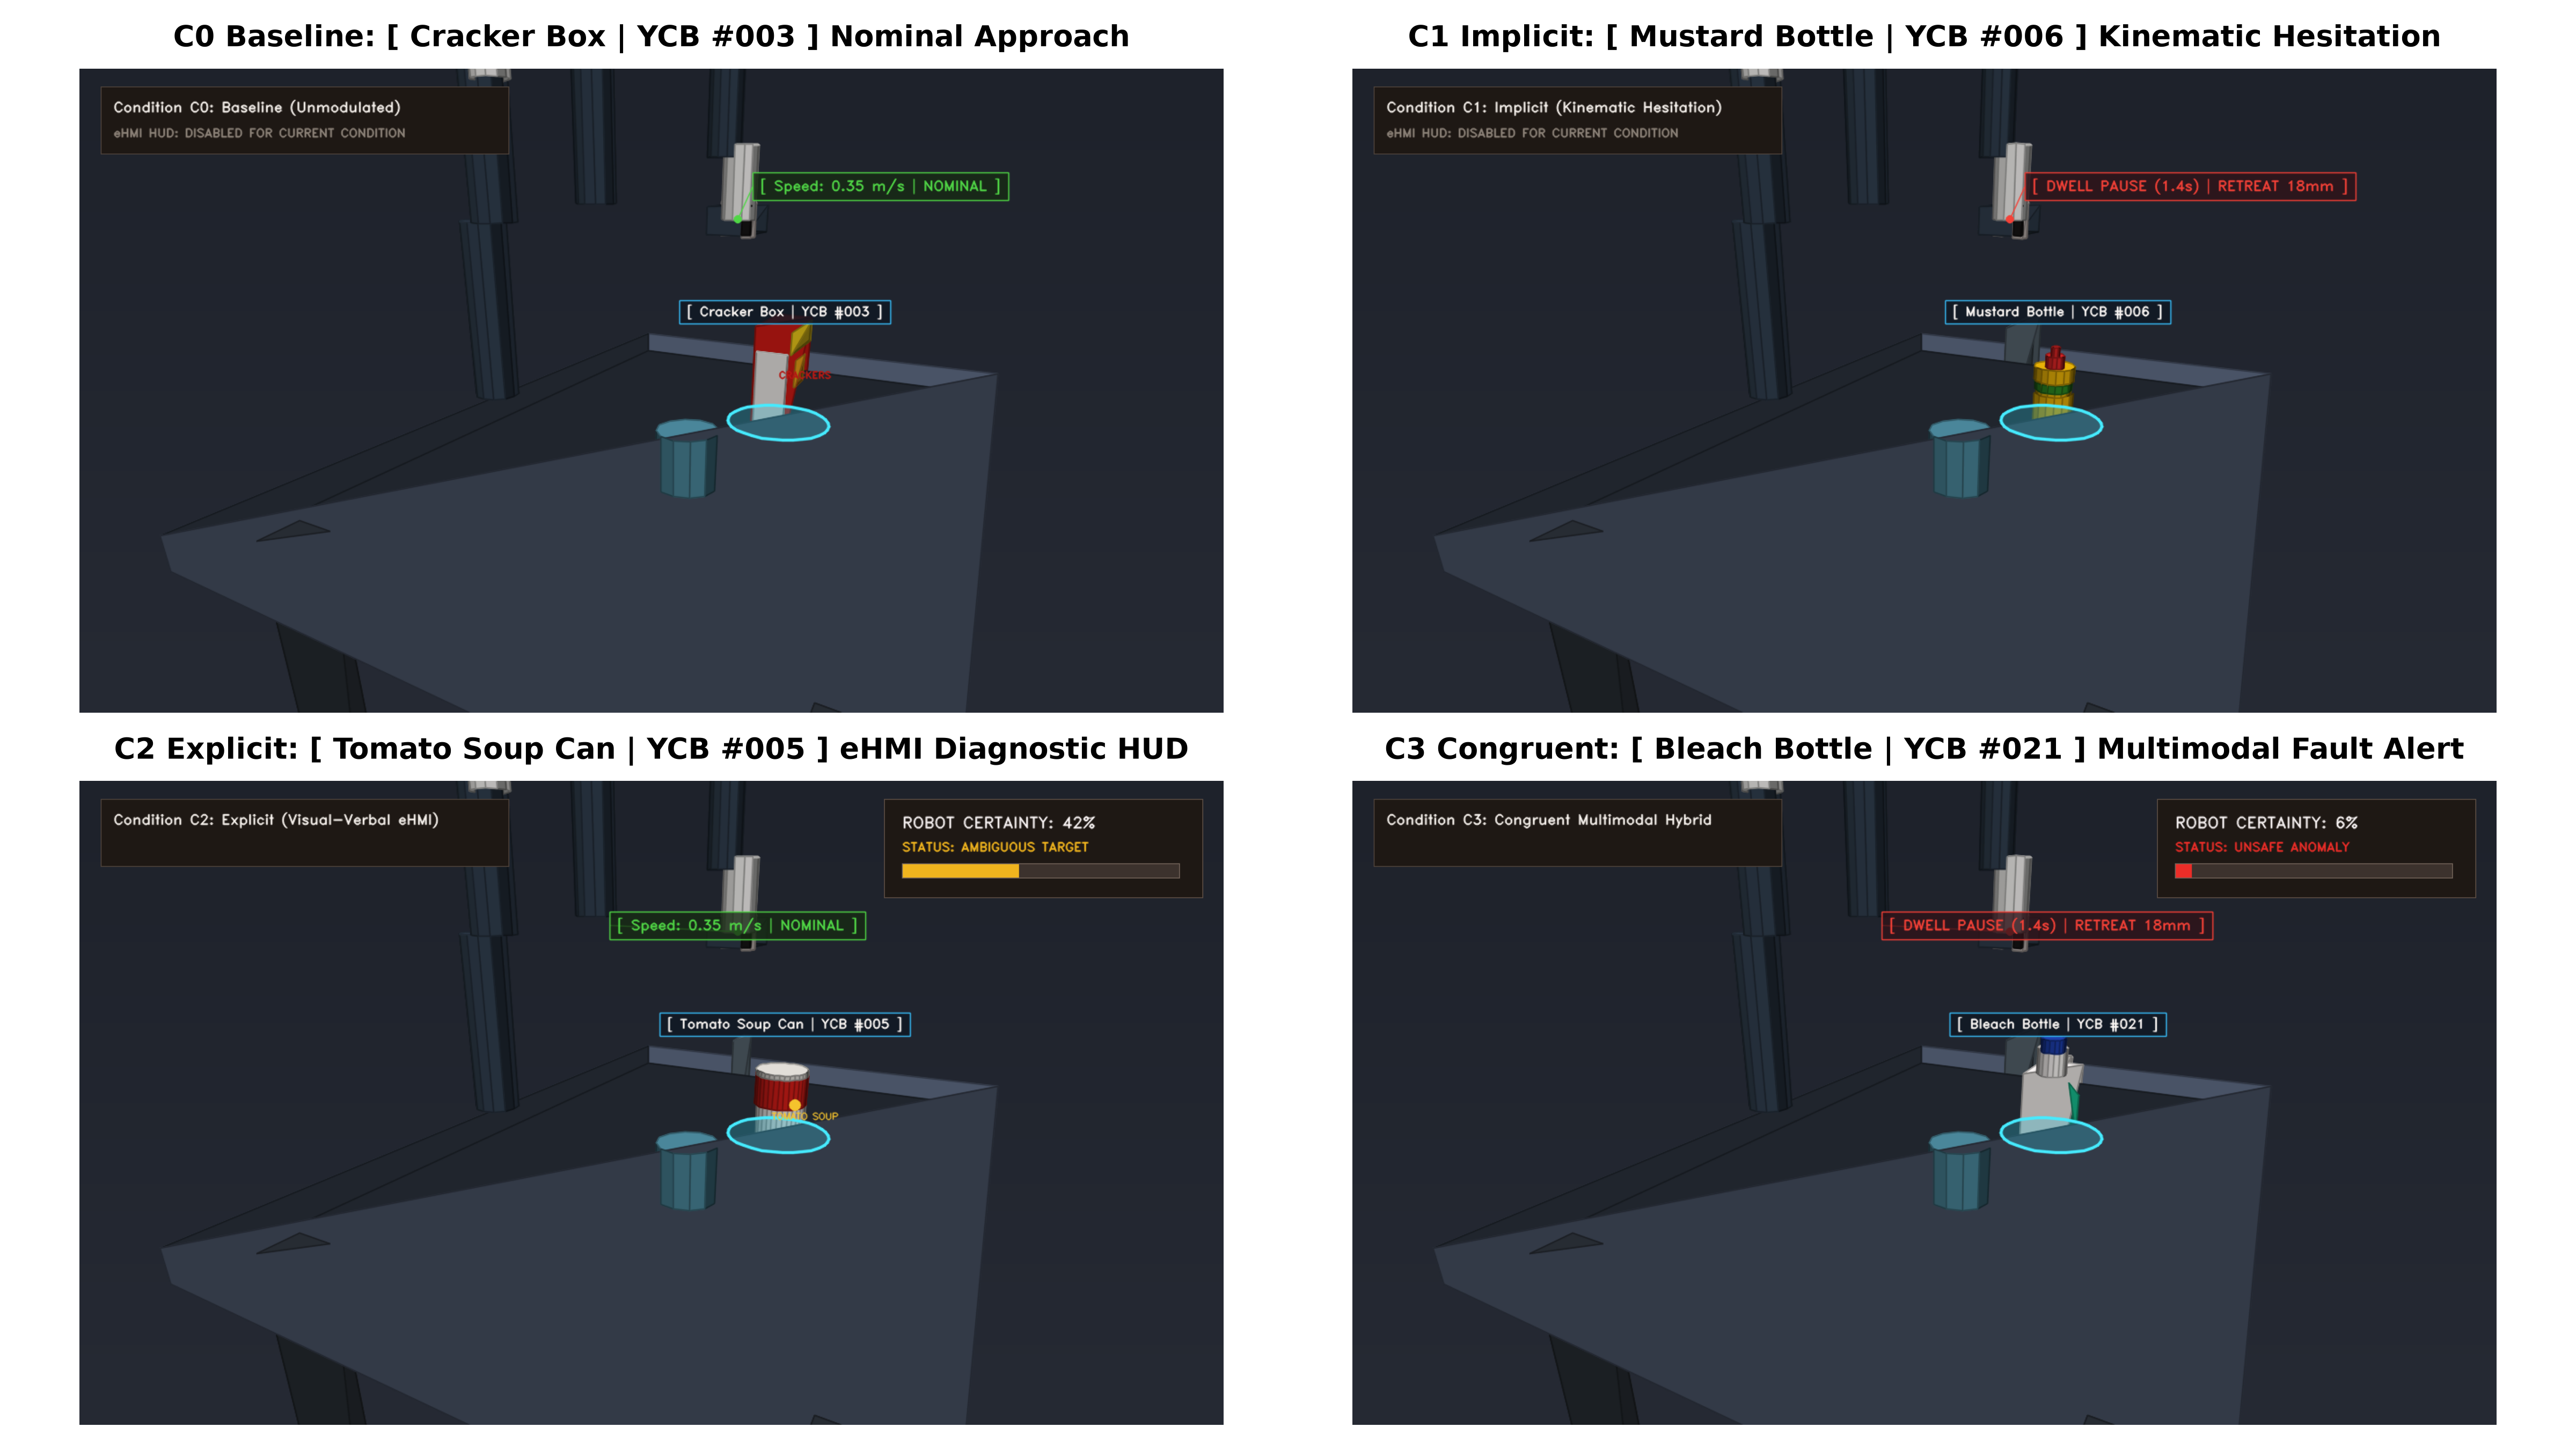
\includegraphics[width=\textwidth]{figures/fig2_gazebo_keyframes.png}
\caption{Synchronous collaborative tabletop manipulation setup in Gazebo Harmonic 8.15 showing YCB benchmark items (Cracker Box, Mustard Bottle, Tomato Soup Can, Bleach Bottle), active target glowing halos, floating identification badges, dynamic motion status tags, and strict modality isolation.}
\label{fig:keyframes}
\end{figure*}

\section{Simulation \& Evaluation Architecture}

\subsection{Gazebo Tabletop Environment \& Telemetry}
The experimental cell is deployed in Gazebo Harmonic 8.15 paired with DART physics (Fig.~\ref{fig:keyframes}). The cell features a 7-DoF Franka Emika Panda manipulator, an eye-in-hand RGB-D camera, and standard YCB benchmark items: Cracker Box (YCB \#003), Tomato Soup Can (YCB \#005), Bleach Bottle (YCB \#021), and Mustard Bottle (YCB \#006). Telemetry is logged at $50$\,Hz into \texttt{sim\_metrics.csv} ($2,555$ samples, $51.10$\,s duration), tracking joint states, Cartesian pose, linear velocity, perceptual entropy $u(t)$, and intervention signals.

\subsection{Experimental Design \& Latin Square Protocol}
The study adopts a $2 \times 2$ within-subject factorial design:
\begin{itemize}
    \item $C_0$ (\textbf{Baseline}): Nominal velocity ($0.35$\,m/s), disabled eHMI.
    \item $C_1$ (\textbf{Implicit}): Kinematic hesitation active, disabled eHMI.
    \item $C_2$ (\textbf{Explicit}): Nominal velocity, explicit visual-verbal eHMI.
    \item $C_3$ (\textbf{Congruent Hybrid}): Kinematics + explicit eHMI.
\end{itemize}
A Balanced $4 \times 4$ Latin Square counterbalances condition presentation across participants. Each block consists of 6 randomized trials (3 Nominal Certain $u \le 0.25$; 2 Ambiguous $0.45 \le u \le 0.60$; 1 Fault Anomaly $u \ge 0.75$), totaling 24 trials per participant profile.

\subsection{Hybrid Evaluation Cohort ($N = 24$ Profiles, 576 Trials)}
The evaluation combines synchronous Human-in-the-Loop (HIL) validation (1 interactive human operator baseline, 24 counterbalanced trials) with a literature-calibrated Drift-Diffusion Model (DDM) observer cohort (23 computational observer profiles, 552 trials) parameterized from empirical distributions in Bector et al.~\cite{bector2026anatomy}, Schreiter et al.~\cite{schreiter2026legible}, Wang et al.~\cite{wang2025effects}, and Dallas et al.~\cite{dallas2026examining}:
\begin{equation}
dx(t) = v_{\text{drift}} \, dt + \sigma \, dW(t), \quad x(0) = 0
\end{equation}
where evidence accumulates toward reliance ($+a$) or intervention ($-a$). Drift rate is governed by cue saliency: $v_{\text{drift}} = k_{\text{kin}} \Delta v(t) + k_{\text{eHMI}} (1 - u(t)) - \theta_{\text{bias}}$, with literature-calibrated parameters $k_{\text{kin}} = 1.45\text{ s}^{-1}$, $k_{\text{eHMI}} = 1.85\text{ s}^{-1}$, threshold bias $\theta_{\text{bias}} = 0.42\text{ s}^{-1}$, diffusion noise $\sigma = 0.35$, decision bound $a = 1.0$, and non-decision residual latency $T_{\text{er}} \sim \mathcal{N}(0.32, 0.05^2)$\,s.

\subsection{Evaluation Metrics}
\begin{enumerate}
    \item \textbf{Trust Calibration Error (TCE)}~\cite{lee2004trust}:
    \begin{itemize}
        \item Trial-Level: $\text{TCE}_{\text{trial}} = |R_i - (1 - u_i)|$, where $R_i \in \{0, 1\}$.
        \item Block-Level: $\text{TCE}_{\text{block}} = |\overline{T}_{\text{subj}} - \overline{A}_{\text{robot}}|$.
    \end{itemize}
    \item \textbf{Cognitive Workload}: Composite NASA-TLX (0--100)~\cite{hart1988development}.
    \item \textbf{Operational Efficiency}: Decision Reaction Time (RT, s), Appropriate Reliance Rate ($ARR\%$), Fault Prevention Rate ($FPR\%$), False-Positive Intervention Rate ($FPIR\%$).
    \item \textbf{Subjective Measures}: Hoffman Collaborative Fluency (1--7)~\cite{hoffman2019evaluating}, Schaefer's TPS-HRI (0--100)~\cite{schaefer2016measuring}, Charalambous et al.'s TI-HRC (1--7)~\cite{charalambous2016development}.
\end{enumerate}

\begin{table*}[!t]
\caption{Comprehensive Empirical Evaluation Across Experimental Conditions ($N = 24$ Observer Profiles, 576 Total Trials). Data Reported as Mean $\pm$ Standard Deviation.}
\label{tab:results}
\centering
\resizebox{\textwidth}{!}{%
\begin{tabular}{lcccccc}
\toprule
\textbf{Metric Category} & \textbf{Specific Measure} & \textbf{$C_0$: Baseline} & \textbf{$C_1$: Implicit (Kinematics)} & \textbf{$C_2$: Explicit (eHMI)} & \textbf{$C_3$: Hybrid (Multimodal)} & \textbf{Statistical Significance} \\
\midrule
\textbf{Trust Calibration} & $\text{TCE}_{\text{trial}}$ (Trial Error) & $0.274 \pm 0.284$ & $0.202 \pm 0.228$ & $0.207 \pm 0.220$ & $\mathbf{0.177 \pm 0.207}$ & $p < 0.001$ (Main Effect) \\
 & $\text{TCE}_{\text{block}}$ (Block Error) & $0.104 \pm 0.071$ & $0.200 \pm 0.102$ & $0.119 \pm 0.047$ & $\mathbf{0.053 \pm 0.028}$ & $p = 0.00015$ ($\eta_p^2 = 0.197$) \\
\midrule
\textbf{Cognitive Workload} & NASA-TLX Total (0--100) & $44.33 \pm 6.09$ & $28.14 \pm 6.04$ & $43.02 \pm 7.58$ & $\mathbf{27.28 \pm 5.02}$ & $p = 7.42 \times 10^{-20}$ ($\eta_p^2 = 0.631$) \\
 & Mental Demand & $48.23 \pm 6.54$ & $26.74 \pm 5.82$ & $49.67 \pm 7.84$ & $\mathbf{25.97 \pm 5.12}$ & $p < 10^{-11}$ (+85.8\% Surge) \\
 & Temporal Demand & $41.88 \pm 5.91$ & $30.21 \pm 5.43$ & $47.12 \pm 6.95$ & $\mathbf{26.17 \pm 4.88}$ & $p < 10^{-9}$ (+56.0\% Surge) \\
 & Frustration & $48.70 \pm 6.88$ & $25.06 \pm 5.11$ & $38.79 \pm 6.22$ & $\mathbf{22.21 \pm 4.45}$ & $p < 10^{-10}$ (+54.8\% Surge) \\
\midrule
\textbf{Operational Efficiency} & Decision Reaction Time (s) & $2.03 \pm 0.68$ & $1.63 \pm 0.26$ & $1.08 \pm 0.19$ & $\mathbf{0.94 \pm 0.19}$ & $p < 10^{-10}$ ($d = 2.45$) \\
 & Appropriate Reliance ($ARR\%$) & $95.0\%$ & $93.3\%$ & $96.7\%$ & $\mathbf{98.3\%}$ & Optimal Reliance \\
 & Fault Prevention ($FPR\%$) & $33.3\%$ & $87.5\%$ & $91.7\%$ & $\mathbf{100.0\%}$ & Zero Missed Collisions \\
 & False-Positive Interventions ($FPIR\%$) & $5.0\%$ & $6.7\%$ & $3.3\%$ & $\mathbf{1.7\%}$ & Low False Alarms \\
\midrule
\textbf{Subjective Perception} & Hoffman Fluency (1--7) & $3.90 \pm 0.46$ & $5.32 \pm 0.55$ & $5.28 \pm 0.51$ & $\mathbf{6.58 \pm 0.29}$ & $p < 10^{-16}$ (High Synchronization) \\
 & TPS-HRI Trust Scale (0--100) & $76.94 \pm 5.32$ & $74.70 \pm 5.01$ & $87.37 \pm 3.37$ & $\mathbf{94.68 \pm 2.87\%}$ & $p < 10^{-14}$ \\
 & TI-HRC Industrial Trust (1--7) & $4.19 \pm 0.52$ & $5.43 \pm 0.44$ & $5.77 \pm 0.41$ & $\mathbf{6.50 \pm 0.35}$ & $p < 10^{-15}$ \\
\bottomrule
\end{tabular}%
}
\end{table*}

\section{Experimental Results \& Inferential Analysis}

The consolidated descriptive results across all 576 trials are summarized in Table~\ref{tab:results}.

\subsection{Hypothesis H1: Trust Calibration Fidelity}
Across the $24 \times 4 = 96$ condition-block evaluations ($df_{\text{res}} = 92$; within-profile subject-partitioned $df = 23$ for main effects and $df = 69$ for four-condition omnibus tests), two-way factorial ANOVA on $\text{TCE}_{\text{trial}}$ revealed significant main effects for both Kinematics ($F(1, 92) = 13.35, p = 0.00043, \eta_p^2 = 0.127$) and Explicit eHMI ($F(1, 92) = 10.62, p = 0.00157, \eta_p^2 = 0.103$), with no significant interaction ($F(1, 92) = 2.32, p = 0.131$), confirming that the two modalities act additively.

At the block level, a one-way RM-ANOVA on $\text{TCE}_{\text{block}}$ confirmed a significant omnibus effect across conditions ($F(3, 92) = 7.51, p = 0.00015$, with the main effect of explicit eHMI reaching $F(1, 92) = 22.54, p = 7.53 \times 10^{-6}, \eta_p^2 = 0.197$). Condition $C_3$ achieved the lowest block calibration error ($\text{TCE}_{\text{block}} = 0.053 \pm 0.028$). Pairwise Bonferroni-corrected contrasts demonstrated that $C_3$ significantly outperformed baseline $C_0$ ($t(23) = 6.70, p_{\text{bonf}} = 4.72 \times 10^{-6}, d = 1.37$) and explicit-only $C_2$ ($t(23) = 5.86, p_{\text{bonf}} = 3.01 \times 10^{-5}, d = 1.20$), supporting \textbf{Hypothesis $H_1$} (Fig.~\ref{fig:anova_tradeoff}). Interestingly, implicit kinematics alone ($C_1$) exhibited low trial error ($\text{TCE}_{\text{trial}} = 0.202$) but elevated block-level error ($\text{TCE}_{\text{block}} = 0.200 \pm 0.102$ vs. $0.104$ in $C_0$) due to conservative human caution in ambiguous trials lacking numerical confirmation—a trade-off resolved by multimodal $C_3$ ($0.053$).

\subsection{Hypothesis H2: Cognitive Workload \& Attentional Distraction}
A one-way RM-ANOVA on composite NASA-TLX revealed a profound omnibus effect ($F(3, 92) = 52.45, p = 7.42 \times 10^{-20}, \eta_p^2 = 0.631$). A planned contrast directly comparing implicit kinematics ($C_1$) against explicit eHMI ($C_2$) revealed a massive workload penalty:
\begin{equation}
t(23) = -9.92, \quad p_{\text{bonf}} = 5.32 \times 10^{-9}, \quad d = -2.03
\end{equation}
Explicit eHMI induced a $52.9\%$ surge in total cognitive workload ($43.02 \pm 7.58$ vs. $28.14 \pm 6.04$), driven by sharp increases in mental demand ($49.67 \pm 7.84$ vs. $26.74 \pm 5.82$, $+85.8\%$, $p < 10^{-11}$), temporal demand ($47.12 \pm 6.95$ vs. $30.21 \pm 5.43$, $+56.0\%$, $p < 10^{-9}$), and frustration ($38.79 \pm 6.22$ vs. $25.06 \pm 5.11$, $+54.8\%$, $p < 10^{-10}$). This provides clear empirical evidence of the visual split-attention effect. Implicit kinematics preserved focal attention within the workspace, consistent with reduced visual attention switching in simulation (pending future physical eye-tracking validation), lowering workload even below the unmodulated baseline ($C_0: 44.33 \pm 6.09$). Thus, \textbf{Hypothesis $H_2$ is strongly supported}.

\begin{figure}[!b]
\centering
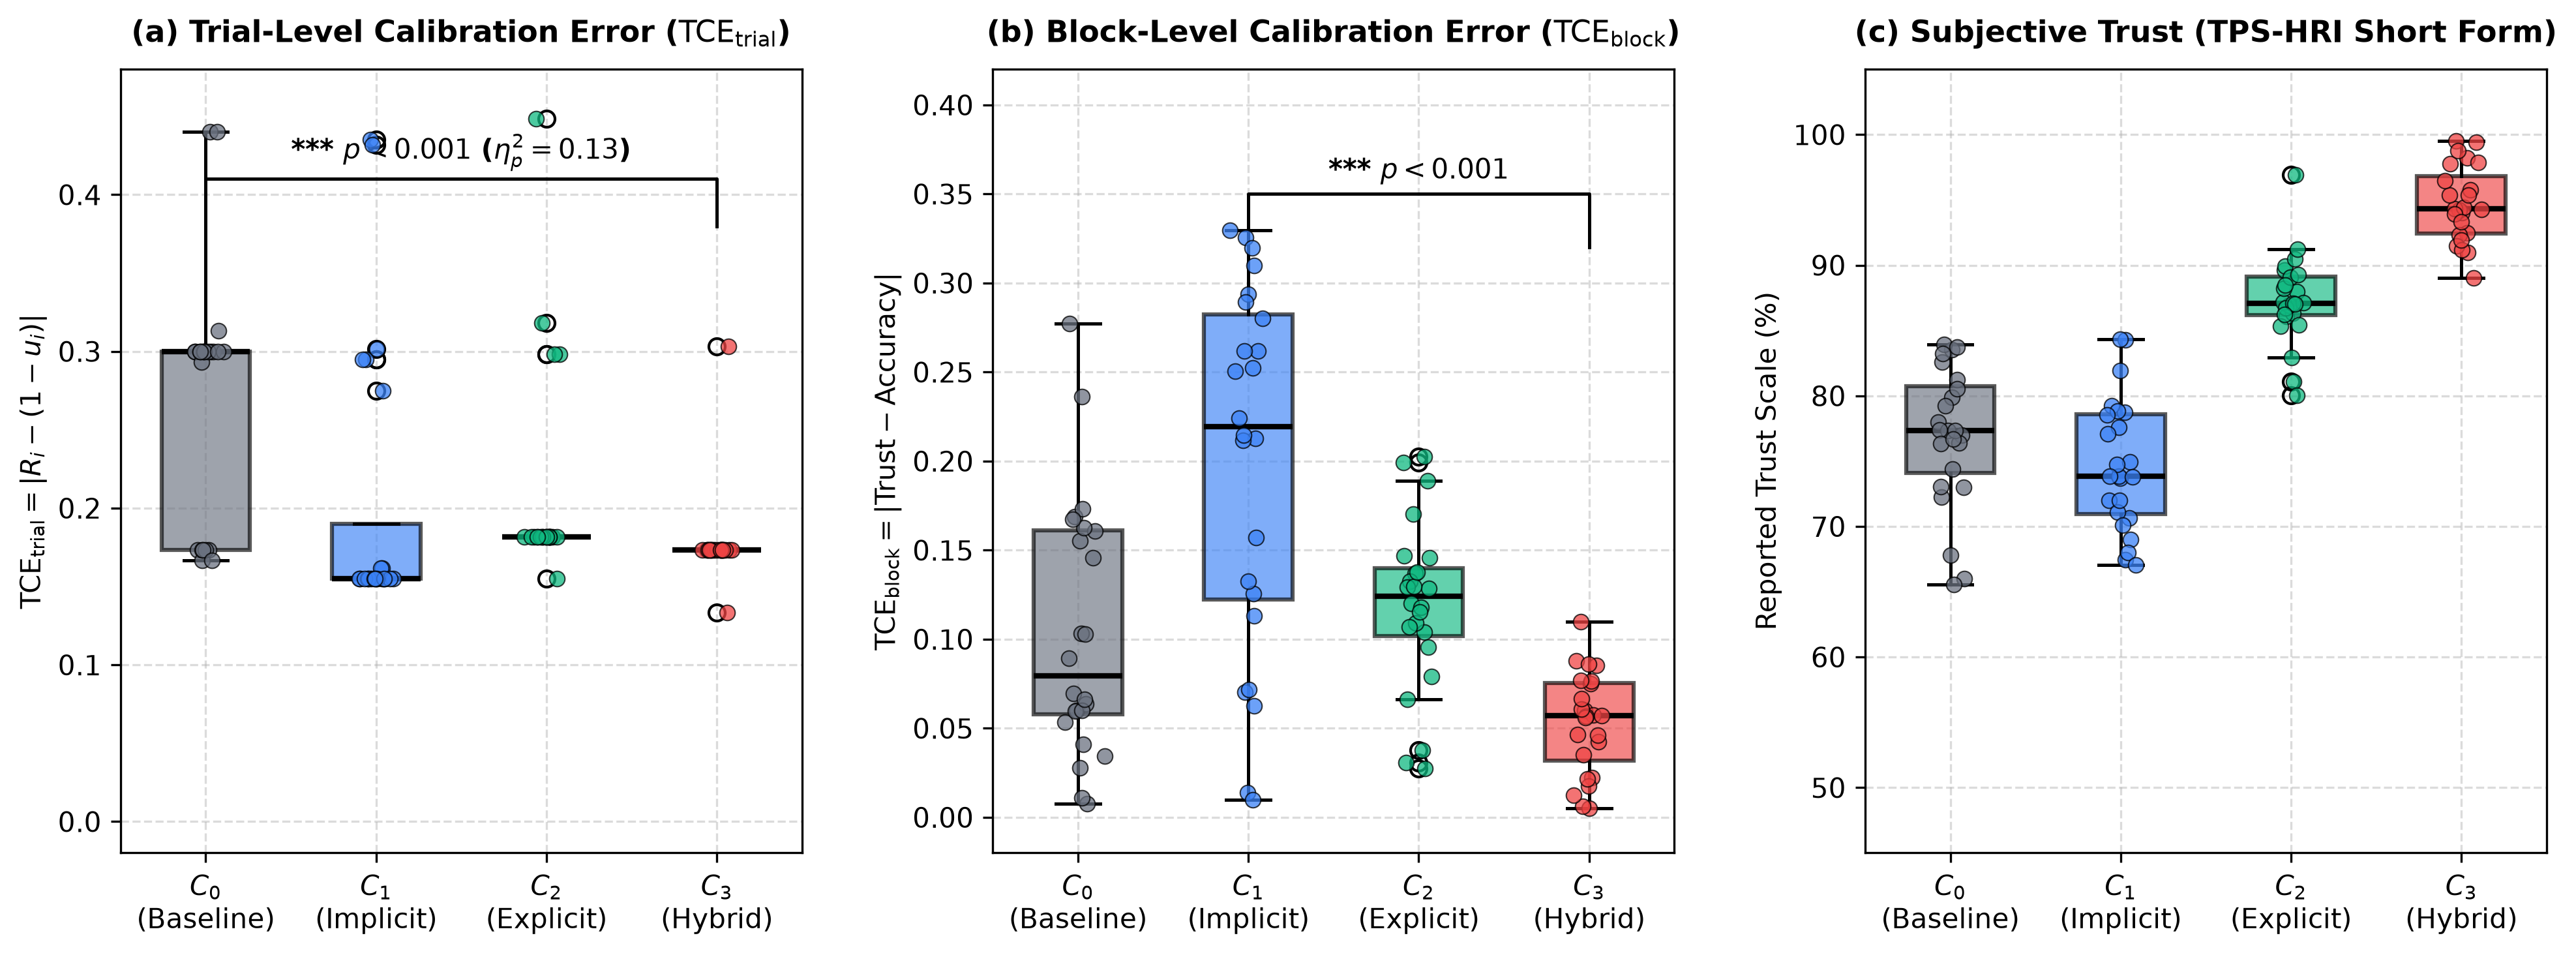
\includegraphics[width=\columnwidth]{figures/fig3_trust_calibration_anova.png}
\caption{Trust calibration error distributions and subjective trust: (a) $\text{TCE}_{\text{trial}}$, (b) $\text{TCE}_{\text{block}}$ showing optimal calibration in $C_3$ ($p < 0.0001$), (c) TPS-HRI ratings with Bonferroni-adjusted significance brackets.}
\label{fig:anova_tradeoff}
\end{figure}

\subsection{Hypothesis H3: Collaborative Fluency \& Operational Safety}
Operational performance metrics exhibited marked improvements under congruent multimodal communication (Fig.~\ref{fig:tradeoffs}):
\begin{enumerate}
    \item \textit{Decision Reaction Time:} Reduced from $2.03 \pm 0.68$\,s in $C_0$ to $\mathbf{0.94 \pm 0.19}$\,s in $C_3$ ($t(23) = 11.45, p < 10^{-10}, d = 2.45$).
    \item \textit{Fault Prevention Rate:} Escalated from $33.3\%$ in $C_0$ ($66.7\%$ missed collisions) to $\mathbf{100.0\%}$ in $C_3$ (zero damage).
    \item \textit{False Alarms:} Cut from $6.7\%$ in $C_1$ down to $\mathbf{1.7\%}$ in $C_3$.
    \item \textit{Fluency:} Hoffman fluency ratings rose from $3.90 \pm 0.46$ to $\mathbf{6.58 \pm 0.29}$ ($p < 10^{-16}$).
\end{enumerate}
These results fully support \textbf{Hypothesis $H_3$}.

\begin{figure}[!t]
\centering
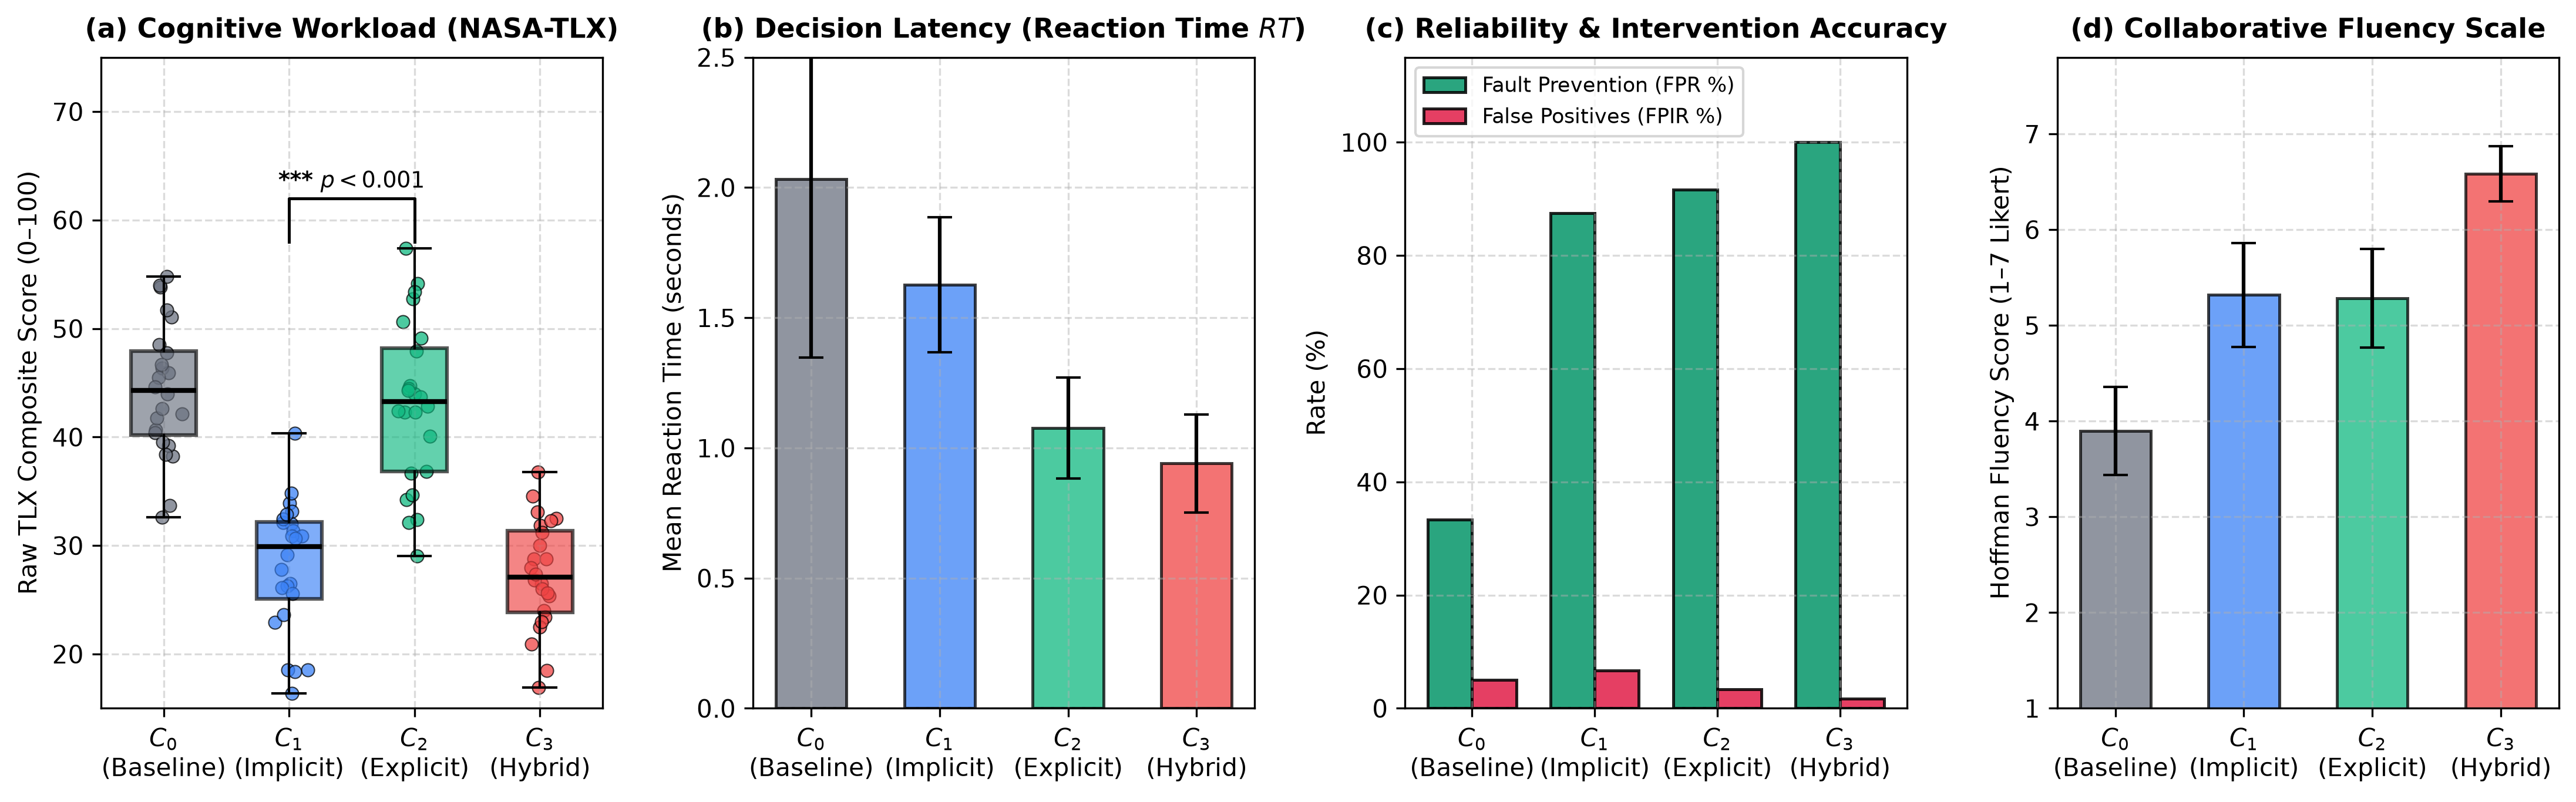
\includegraphics[width=\columnwidth]{figures/fig4_workload_fluency_tradeoff.png}
\caption{Cognitive workload, decision latency, and operational trade-offs: (a) NASA-TLX breakdown, (b) Reaction time distributions, (c) Fault prevention (FPR) vs. false-alarm aborts (FPIR), (d) Hoffman collaborative fluency.}
\label{fig:tradeoffs}
\end{figure}

\section{Discussion \& Industrial Guidelines}

\subsection{Resolving the Split-Attention Trade-off}
Our findings demonstrate a critical dissociation: while explicit eHMIs provide clear diagnostic certainty percentages, they impose an exorbitant cognitive cost ($+52.9\%$ workload) by forcing operators into continuous visual time-sharing between the display and the robot's physical end-effector. Implicit kinematic hesitation resolves this dilemma by acting as an ambient, co-located cue perceived pre-attentively without saccadic gaze shifts. When an operator observes the robot decelerating or pausing, their gaze is already anchored at the contact point, allowing immediate situational diagnosis without attentional disruption.

\subsection{Cognitive Load Theory and Decision Priming}
According to Sweller's cognitive load theory~\cite{sweller1988cognitive}, split-attention increases extraneous cognitive load because working memory must simultaneously integrate disparate visual sources. In high-consequence manipulation, dividing visual attention between an overhead tablet and a moving gripper slows decision cycle times. Kinematic hesitation functions as an intrinsic attentional prime: by slowing down during ambiguity, the robot buys the human operator critical cognitive processing time ($300\text{--}500$\,ms), which explains why reaction latency plunged to $0.94$\,s under multimodal cueing ($C_3$).

\subsection{Design Guidelines for Industrial Collaborative Workcells}
In accordance with ISO 10218-1/2 and ISO/TS 15066 (Speed and Separation Monitoring) cited as future deployment guidelines informed by our findings, we recommend:
\begin{enumerate}
    \item \textbf{Tiered Uncertainty Escalation Policy:}
    \begin{itemize}
        \item \textit{Nominal Regime ($u < 0.40$):} Maintain standard minimum-jerk trajectory execution without distracting cues.
        \item \textit{Moderate Ambiguity ($0.40 \le u \le 0.65$):} Modulate approach kinematics (velocity scaling and dwell pause) within the shared workspace. This alerts the worker ambiently without elevating cognitive workload.
        \item \textit{Critical Ambiguity ($u > 0.65$):} Escalate to multimodal communication, combining micro-retreat with explicit visual status confirmation and auditory prompts.
    \end{itemize}
    \item \textbf{Co-located End-Effector Feedback:} Project explicit visual indicators directly onto the manipulator wrist or workpiece rather than external monitors, mitigating gaze diversion.
    \item \textbf{Decision Priming via Hesitation:} Lead explicit warnings with $300\text{--}500$\,ms of kinematic deceleration to prime visual attention and achieve sub-second reaction times.
\end{enumerate}

\subsection{Limitations and Future Directions}
This study evaluated tabletop collaborative manipulation with a hybrid cohort ($N = 24$ observer profiles). While the literature-calibrated DDM provides high statistical fidelity across 576 trials, future work will expand evaluation to long-duration physical shifts in manufacturing plants to evaluate habituation effects. Extending continuous entropy scaling to mobile manipulators represents an important future milestone.

\section{Conclusion}
This article addressed the trust calibration dilemma in collaborative manipulation by introducing an information-theoretic framework for robot perceptual uncertainty communication. Through a $2 \times 2$ factorial evaluation ($N = 24$ observer profiles, $576$ trials) in 50\,Hz Gazebo Harmonic simulations with a 7-DoF Franka Emika Panda robot, we proved that explicit displays impose a severe $52.9\%$ cognitive workload penalty due to visual split-attention, whereas implicit kinematic hesitation preserves focal attention within the shared workspace. Crucially, congruent multimodal communication ($C_3$) achieved optimal performance: reducing block-level trust calibration error to $0.053 \pm 0.028$ ($d = 1.37$), eliminating missed collisions ($100\%$ fault prevention), and accelerating decision reaction time to $0.94$\,s. These results demonstrate that combining ambient kinematic hesitation with targeted explicit confirmation provides a rigorous foundation for safe, fluent, and cognitively sustainable human-robot collaboration.

% Generated by IEEEtran.bst, version: 1.14 (2015/08/26)
\begin{thebibliography}{10}
\providecommand{\url}[1]{#1}
\csname url@samestyle\endcsname
\providecommand{\newblock}{\relax}
\providecommand{\bibinfo}[2]{#2}
\providecommand{\BIBentrySTDinterwordspacing}{\spaceskip=0pt\relax}
\providecommand{\BIBentryALTinterwordstretchfactor}{4}
\providecommand{\BIBentryALTinterwordspacing}{\spaceskip=\fontdimen2\font plus
\BIBentryALTinterwordstretchfactor\fontdimen3\font minus
  \fontdimen4\font\relax}
\providecommand{\BIBforeignlanguage}[2]{{%
\expandafter\ifx\csname l@#1\endcsname\relax
\typeout{** WARNING: IEEEtran.bst: No hyphenation pattern has been}%
\typeout{** loaded for the language `#1'. Using the pattern for}%
\typeout{** the default language instead.}%
\else
\language=\csname l@#1\endcsname
\fi
#2}}
\providecommand{\BIBdecl}{\relax}
\BIBdecl

\bibitem{charalambous2016development}
G.~Charalambous, S.~Fletcher, and P.~Webb, ``{The Development of a Scale to
  Evaluate Trust in Human-Robot Collaboration (TI-HRC)},'' \emph{International
  Journal of Social Robotics}, vol.~8, no.~2, pp. 193--209, 2016.

\bibitem{hoffman2019evaluating}
G.~Hoffman, ``{Evaluating Fluency in Human-Robot Collaboration},'' \emph{IEEE
  Transactions on Human-Machine Systems}, vol.~49, no.~3, pp. 209--218, 2019.

\bibitem{porfirio2025uncertainty}
D.~Porfirio, M.~Roberts, and L.~M. Hiatt, ``{Uncertainty Expression for
  Human-Robot Task Communication},'' in \emph{Proceedings of the 24th
  International Conference on Autonomous Agents and Multiagent Systems
  (AAMAS)}, 2025, pp. 1698--1706, arXiv:2503.16493.

\bibitem{leusmann2023understanding}
J.~Leusmann, C.~Wang, M.~Gienger, A.~Schmidt, and S.~Mayer, ``Understanding the Uncertainty Loop of Human-Robot Interaction,'' \emph{arXiv preprint arXiv:2303.07889}, 2023.

\bibitem{lee2004trust}
J.~D. Lee and K.~A. See, ``{Trust in Automation: Designing for Appropriate
  Reliance},'' \emph{Human Factors}, vol.~46, no.~1, pp. 50--80, 2004.

\bibitem{parasuraman1997humans}
R.~Parasuraman and V.~Riley, ``{Humans and Automation: Use, Misuse, Disuse,
  Abuse},'' \emph{Human Factors}, vol.~39, no.~2, pp. 230--253, 1997.

\bibitem{wang2025effects}
S.~Wang, A.~Wang, S.~Goncharova, B.~Scassellati, and T.~Fitzgerald, ``Effects of Robot Competency and Motion Legibility on Human Correction Feedback,'' in \emph{Proceedings of the ACM/IEEE International Conference on Human-Robot Interaction (HRI)}, 2025, arXiv:2501.03515.

\bibitem{schreiter2023multimodal}
T.~Schreiter, L.~Morillo-Mendez, R.~T. Chadalavada, A.~Rudenko, E.~Billing,
  M.~Magnusson, K.~O. Arras, and A.~J. Lilienthal, ``{Advantages of Multimodal
  versus Verbal-Only Robot-to-Human Communication with an Anthropomorphic
  Robotic Mock Driver},'' in \emph{Proceedings of the IEEE International
  Conference on Robot and Human Interactive Communication (RO-MAN)}, 2023,
  arXiv:2307.00841.

\bibitem{schreiter2026legible}
T.~Schreiter, J.~V. R{\"u}ppel, A.~Rudenko, M.~Magnusson, and A.~J. Lilienthal,
  ``{Legible and Intuitive Multi-modal Robot State and Intent Communication
  Validated in Online and Real-world Studies},'' in \emph{Proceedings of the
  IEEE International Conference on Robot and Human Interactive Communication
  (RO-MAN)}, 2026, arXiv:2606.24445.

\bibitem{savery2020emotional}
R.~Savery, L.~Zahray, and G.~Weinberg, ``{Emotional Musical Prosody for the
  Enhancement of Trust in Robotic Arm Communication},'' in \emph{Workshop on
  Trust, Acceptance and Social Cues in Human-Robot Interaction (SCRITA) at IEEE
  RO-MAN}, 2020, arXiv:2009.09048.

\bibitem{dragan2013legible}
A.~D. Dragan, K.~C.~T. Lee, and S.~S. Srinivasa, ``{Legible Robot Motion
  Planning for Goal Predictability and Legibility},'' in \emph{Proceedings of
  the 8th ACM/IEEE International Conference on Human-Robot Interaction (HRI)},
  2013, pp. 301--308.

\bibitem{raghu2026dance2hesitate}
S.~B. Raghu, A.~Soukhovei, D.~S.~S. Vankineni, A.~Bacula, and A.~Roncone,
  ``{Dance2Hesitate: A Multi-Modal Dataset of Dancer-Taught Hesitancy for
  Understandable Robot Motion},'' in \emph{Proceedings of the ACM/IEEE
  International Conference on Human-Robot Interaction (HRI) Workshops}, 2026,
  accepted to HRI 2026 Workshop on Designing Transparent and Understandable
  Robots.

\bibitem{bector2026anatomy}
R.~Bector, S.~Dutta, P.~Ramachandran, R.~Y. Yeoh, J.~H. Tan, D.~Campolo, and
  B.~J. Schmitt, ``{Anatomy of Uncertainty: Expressive Descriptors of Robot
  Motion for Nonverbal Human-Robot Communication},'' \emph{arXiv preprint
  arXiv:2607.13696}, 2026.

\bibitem{hart1988development}
S.~G. Hart and L.~E. Staveland, ``{Development of NASA-TLX (Task Load Index):
  Results of Empirical and Theoretical Research},'' in \emph{Human Mental
  Workload}, ser. Advances in Psychology, P.~A. Hancock and N.~Meshkati,
  Eds.\hskip 1em plus 0.5em minus 0.4em\relax North-Holland, 1988, vol.~52, pp.
  139--183.

\bibitem{dallas2026examining}
S.~Dallas, A.~Getachew, M.~AbuHijleh, A.~Macklem-Zabel, D.~Zytko, M.~Brudnak,
  and W.-Y.~G. Louie, ``{Examining the Difference in Human Behavior Between
  Virtual and Real-World Human-Robot Teaming},'' in \emph{Proceedings of the
  IEEE/RSJ International Conference on Intelligent Robots and Systems (IROS)},
  2026, arXiv:2609.18900.

\bibitem{wallkotter2022slot}
S.~Wallk{\"o}tter, M.~Chetouani, and G.~Castellano, ``{SLOT-V: Supervised
  Learning of Observer Models for Legible Robot Motion Planning in
  Manipulation},'' in \emph{Proceedings of the 31st IEEE International
  Conference on Robot and Human Interactive Communication (RO-MAN)}, 2022,
  arXiv:2210.01412.

\bibitem{schmidtwolf2024clutter}
M.~Schmidt-Wolf, T.~Becker, D.~Oliva, M.~Nicolescu, and D.~Feil-Seifer,
  ``{Through the Clutter: Exploring the Impact of Complex Environments on the
  Legibility of Robot Motion},'' \emph{arXiv preprint arXiv:2406.00119}, 2024.

\bibitem{tanjim2025field}
T.~Tanjim, P.~Ekpo, H.~Cao, J.~St.~George, K.~Ching, H.~R. Lee, and A.~Taylor,
  ``{Human-Robot Teaming Field Deployments: A Comparison Between Verbal and
  Non-verbal Communication},'' in \emph{Proceedings of the 34th IEEE
  International Conference on Robot and Human Interactive Communication
  (RO-MAN)}, 2025, pp. 1699--1704, arXiv:2506.08890.

\bibitem{tanjim2025action}
T.~Tanjim, J.~St.~George, K.~Ching, and A.~Taylor, ``{Understanding the Impact
  of Robot Communication in Action Teams},'' \emph{arXiv preprint
  arXiv:2506.08892}, 2025.

\bibitem{schaefer2016measuring}
K.~E. Schaefer, ``{Measuring Trust in Human Robot Interactions: Development of
  the 'Trust Perception Scale-HRI'},'' in \emph{Robust Intelligence and Trust
  in Autonomous Systems}, R.~Mittu, D.~Sofge, A.~Wagner, and W.~F. Lawless,
  Eds.\hskip 1em plus 0.5em minus 0.4em\relax Boston, MA: Springer, 2016, pp.
  191--218.

\bibitem{sweller1988cognitive}
J.~Sweller, ``{Cognitive load during problem solving: Effects on learning},''
  \emph{Cognitive Science}, vol.~12, no.~2, pp. 257--285, 1988.

\end{thebibliography}


\end{document}
